\documentclass{article}
\usepackage[utf8]{inputenc}
\usepackage{imakeidx}
\usepackage[italian]{babel}
\usepackage{graphicx}
\usepackage[T1]{fontenc}
\makeindex
\usepackage{float}
%\graphicspath{}
\title{Oscillatore di Collpits}
\author{William Perri 4427140 }
\setlength{\parskip}{1em}
\renewcommand{\baselinestretch}{1.2}
%\DeclareGraphicsExtensions{.jpeg,.png}
\date{27/06/2020}

\begin{document}

\maketitle
Insegnamento di LABORATORIO DI ELETTRONICA A.A. 2019/20

\newpage
\tableofcontents
\newpage
\section{Introduzione}
Lo scopo di questo progetto è quello di realizzare un oscillatore di Collpits, ma per iniziare dovremmo definire innanzitutto cosa è un oscillatore.
Un oscillatore (sinusoidale) è caratterizzato da:
\begin{itemize}
\item Frequenza
\item Ampiezza
\item stabilità in frequenza
\item stabilità in ampiezza
\item purezza spettrale
\item contenuto armonico
\end{itemize}
In seguito andremo ad analizzare ogni singolo punto della lista in particolar modo riferito all'oscillatore di Collpits.
\newpage
\section{Descrizione del Progetto}
\subsection{La frequenza di oscillazione}
~\begin{figure}[H]
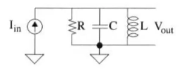
\includegraphics[scale=1]{RisonatoreParallelo.png} 
\caption{Schema circuitale di un risonatore parallelo}
\label{fig:foo}
\end{figure}
In questa figura è mostrato il risonatore parallelo, l'ammettenza del circuito vale 
$Y=G+j\omega C+\frac{1}{j\omega L}=G+j(\omega C-\frac{1}{\omega L}$ da cui $\omega_0C-\frac{1}{\omega _0L})=0\\Rightarrow\omega _0=\frac{1}{\sqrt{LC}}$ dove $\omega _0$ è la frequenza di risonanza, G è la conduttanza del resistore, gli altri due termini sono le reattanze dei due elementi reattivi.
Alla risonanza le correnti del capacitore e dell'induttore si "annullano" a vicenda,per cui dal generatore viene vista solo la resistenza. 
\subsection{La purezza spettrale}
Facendo un analisi in frequenza della forma d'onda generata da un oscillatore, dovremmo vedere una linea verticale in corrispondenza della frequenza di oscillazione e zero altrove, tuttavia questo non è possibile dal punto di vista pratico, lo spettro di un oscillatore reale mostra che c'è della potenza anche in un intorno più o meno stretto della frequenza centrale.
Questo concetto viene definito rumore di fase.

~\begin{figure}[H]
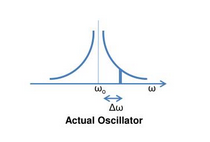
\includegraphics[scale=1]{PhaseNoise.png} 
\caption{Spettro di un oscillatore reale.}
\label{fig:foo}
\end{figure}

\subsection{Il fattore di merito}
Il concetto di fattore di merito è l'energia immagazzinata all'interno del risonatore, il momento in cui la corrente è nulla nell'induttore corrisponde a quella in cui la tensione sul condensatore è massima, l'energia del condensatore è $\frac{1}{2}CV^2$.

Quando il condensatore si scarica al minimo, la corrente dell'induttore sarà massima, per cui l'energia sarà contenuta nel campo magnetico dell'induttore determinato da $\frac{1}{2}LI^2$.
Il fattore di merito ci dice quanta di questa energia dissipiamo:

$Q=\omega\frac{EnergiaImmagazzinata}{PotenzaMediaDissipataPerPeriodo}$
\centering

Nella configurazione parallelo vista in precedenza $Q=\frac{1}{\sqrt{LC}}\frac{\frac{1}{2}CV^2}{\frac{1}{2}RI^2}=\frac{R}{\sqrt{\frac{L}{C}}}$.

Dalla prima equazione vista, ovvero quella del calcolo di $\omega_0$ partendo da L e C, e sapendo che la richiesta è far oscillare il nostro sistema a 5MHz, è stato deciso di utilizzare (tra le infinite possibilità di valori) C=100pF e L=10uH per via della facile reperibilità di questi componenti.

Con questi valori possiamo calcolarci l'impedenza caratteristica della rete:
$Z_0=\sqrt{\frac{L}{C}}=316\Omega$
\centering

Più il fattore di merito aumenta e più la curva dello spettro sarà "appuntita", il che vuol dire meno rumore di fase, un oscillatore al quarzo di buona qualità ha un fattore di merito Q=10000, un oscillatore a componenti tradizionali potrebbe arrivare a circa Q=5.

Introduciamo un nuovo concetto: la larghezza di banda dello spettro.

In questo caso si intende la banda in cui lo spettro sta dentro il range di -3dB del massimo.
Facendo un semplice calcolo è possibile vedere che il rapporto tra la larghezza di banda e la frequenza centrale è pari a 1/Q.
Ovviamente questo vuol dire che più la banda è stretta maggiore sarà il fattore di merito.
Il problema di questa realizzazione è che bisogna confrontarsi con i limiti del mondo reale, quindi la resistenza non sarà in parallelo a L e C ma la troveremo in serie a L, perché modelliamo l'induttore reale come un induttore ideale con una resistenza serie.
Ipotizziamo che $RL_S$ e $RL_P$ siano equivalenti, supponendo un Q elevato otteniamo che $R_P=R_S*Q^2$  e $L_p=L_s$.
A questo punto, ricordandoci che L=10uH, $\omega_0=2\pi * 5MHz$, la $R_s$ la andiamo a cercare su un datasheet di un induttore reale e troviamo che è circa $1\Omega$, possiamo calcolarci Q che sarà pari a 316 e per quanto detto prima $R_p=R_sQ^2=10k\Omega$.
%Da fare la lezione del 16/03 da 1h 31m

\newpage
\section{Realizzazione}

\newpage
\section{Risultati}

\newpage

\section{Conclusioni}

\newpage
\section{Riferimenti}

\begin{itemize}
\item The Design of CMOS Radio-Frequency Integrated Circuits - Thomas H. Lee
\item RF Microeletronics - B. Razavi
\end{itemize}
\end{document}
